\documentclass[]{article}
\usepackage[T1]{fontenc}
\usepackage{lmodern}
\usepackage{amssymb,amsmath}
\usepackage{ifxetex,ifluatex}
\usepackage{fixltx2e} % provides \textsubscript
% use microtype if available
\IfFileExists{microtype.sty}{\usepackage{microtype}}{}
% use upquote if available, for straight quotes in verbatim environments
\IfFileExists{upquote.sty}{\usepackage{upquote}}{}
\ifnum 0\ifxetex 1\fi\ifluatex 1\fi=0 % if pdftex
  \usepackage[utf8]{inputenc}
\else % if luatex or xelatex
  \usepackage{fontspec}
  \ifxetex
    \usepackage{xltxtra,xunicode}
  \fi
  \defaultfontfeatures{Mapping=tex-text,Scale=MatchLowercase}
  \newcommand{\euro}{€}
\fi
\usepackage{color}
\usepackage{fancyvrb}
\DefineShortVerb[commandchars=\\\{\}]{\|}
\DefineVerbatimEnvironment{Highlighting}{Verbatim}{commandchars=\\\{\}}
% Add ',fontsize=\small' for more characters per line
\newenvironment{Shaded}{}{}
\newcommand{\KeywordTok}[1]{\textcolor[rgb]{0.00,0.44,0.13}{\textbf{{#1}}}}
\newcommand{\DataTypeTok}[1]{\textcolor[rgb]{0.56,0.13,0.00}{{#1}}}
\newcommand{\DecValTok}[1]{\textcolor[rgb]{0.25,0.63,0.44}{{#1}}}
\newcommand{\BaseNTok}[1]{\textcolor[rgb]{0.25,0.63,0.44}{{#1}}}
\newcommand{\FloatTok}[1]{\textcolor[rgb]{0.25,0.63,0.44}{{#1}}}
\newcommand{\CharTok}[1]{\textcolor[rgb]{0.25,0.44,0.63}{{#1}}}
\newcommand{\StringTok}[1]{\textcolor[rgb]{0.25,0.44,0.63}{{#1}}}
\newcommand{\CommentTok}[1]{\textcolor[rgb]{0.38,0.63,0.69}{\textit{{#1}}}}
\newcommand{\OtherTok}[1]{\textcolor[rgb]{0.00,0.44,0.13}{{#1}}}
\newcommand{\AlertTok}[1]{\textcolor[rgb]{1.00,0.00,0.00}{\textbf{{#1}}}}
\newcommand{\FunctionTok}[1]{\textcolor[rgb]{0.02,0.16,0.49}{{#1}}}
\newcommand{\RegionMarkerTok}[1]{{#1}}
\newcommand{\ErrorTok}[1]{\textcolor[rgb]{1.00,0.00,0.00}{\textbf{{#1}}}}
\newcommand{\NormalTok}[1]{{#1}}
\usepackage{graphicx}
% We will generate all images so they have a width \maxwidth. This means
% that they will get their normal width if they fit onto the page, but
% are scaled down if they would overflow the margins.
\makeatletter
\def\maxwidth{\ifdim\Gin@nat@width>\linewidth\linewidth
\else\Gin@nat@width\fi}
\makeatother
\let\Oldincludegraphics\includegraphics
\renewcommand{\includegraphics}[1]{\Oldincludegraphics[width=\maxwidth]{#1}}
\ifxetex
  \usepackage[setpagesize=false, % page size defined by xetex
              unicode=false, % unicode breaks when used with xetex
              xetex]{hyperref}
\else
  \usepackage[unicode=true]{hyperref}
\fi
\hypersetup{breaklinks=true,
            bookmarks=true,
            pdfauthor={},
            pdftitle={},
            colorlinks=true,
            urlcolor=blue,
            linkcolor=magenta,
            pdfborder={0 0 0}}
\urlstyle{same}  % don't use monospace font for urls
\setlength{\parindent}{0pt}
\setlength{\parskip}{6pt plus 2pt minus 1pt}
\setlength{\emergencystretch}{3em}  % prevent overfull lines
\setcounter{secnumdepth}{0}

\author{}
\date{}

\begin{document}

\subsection{Abstract}

We face a deluge of data that scientists need to deal with in many
different domains today. While there are already good solutions to some
parts of the data life cycle the applicability of the solutions to
certain scientific domains often varies. Especially research domains
with high degree of interdisciplinary interactions and heterogeneity in
methods and data in general like ecology face problems in dealing with
some valuable concepts like ontologies that potentially can be used to
improve or automate some of the most common tasks in analyses like
finding relevant data, cleaning and merging of datasets. We here
introduce the \texttt{rbefata} package that connects to the open source
data management platform \texttt{BEFdata} that has been developed and is
used within the BEF-China experiment. We show the use of the package in
combination with the portal using an example workflow that integrates
three datasets from the BEF-China experiment representing an analysis
that has been published already. We discuss the combination of the R
package \texttt{rbefdata} and the data poral in the context of state of
the art data management as well as we give an outlook on upcoming
features that will bring semantical featues like smart merges based on
an ontology we created.

\subsection{Introduction}

With a growing awareness on the long term value of data, much effort has
been put into building data management platforms, to preserve all kind
of environmental and historic data, over the last years (e.g.~diversity
workbench, BEFdata). Many specialized solutions for different scientific
disciplines appeared that provide data management plans for small scale
projects or collaborations as well as for large data producing long term
or remote sensing projects. An ongoing trend in that context is the
development of integrative databases or data portals. They serve as
nodes that collect data from smaller databases of a certain domain and
they give researchers of that domain the opportunity to access a wide
range of relevant data from one place. This portals in fact offer a
solution to to one of the most pressing problems that we face with our
valuable data today, their lost.

Another big problem with data, especially in terms of reuse of available
data, is the general understanding of datasets. Usually plain datasets
say nothing, to one who is not familiar with it and they are even hard
to decipher by the author itself after some time has passed. It is
usually hard to remember exactly what methods have been used to collect
a certain columns data or what the abbreviations or headers in the
dataset mean. To solve this this problem metadata frameworks have been
developed and published as standards so nobody really needs to think
about an own set of requirements to describe its data. The Ecological
Metadata Language is only one example for that. While this theoretically
solves the problem with not well described datasets it is still hard to
make people use it extensively as this usually always means to learn new
tools that help with the description process (e.g morpho, data up).

While well described data helps a lot in understanding datasets and on
deciding upon the relevance and applicability in a certain analysis
there is still lots of manual intervention necessary after that to
prepare the data for analysis (cite yourself? or xxx). It may needs to
be cleaned, imputed, reshaped and merged which usually takes up to 70\%
of the analysis workflow, before the smart models can be applied to the
data to find interesting patters (cite the workflow paper of Karin and
me). This preparation steps not only are time and labour intensive but
also potentially error prone, especially as the complexity of analyses
grows.

Ontologies, formal representations of knowledge potentially offer a
sophisticated tool to deal with that step of data preparation (cite
supporting ecology as data intensive science). While they are already
used in some research domains like genetics (cite xxx), other domains
face more problems using it. For example in ecology, that has grown into
a very collaborative, interdisciplinary and data intensive science over
the last decade, to address questions on a greater temporal and spatial
scale (e.g michener et al 2012). The data here is mainly provided by
small scale studies spread all over the world (e.g heidorn2009 shedding
light on the dark) but also through bigger long term projects like LTER
(cite xxx), BEF-China (cite xxx), governmental projects and local
initiatives (cite xxx). This in fact results in a wild growing, complex
and heterogeneous data landscape in that we need to deal with. The
application of ontologies in ecology is discussed controversially (cite
xxx) which is mainly related to the heterogeneity of the research domain
and it is argued that they can be a benefit, but it is hard to set up a
sophisticated ontology covering all necessary terms and relation of a
that complex research domain like ecology.

As there is a growing demand to use and reuse available data and to
embed small heterogeneous data into a wider context in ecology we here
introduce the R package \texttt{rbefdata} that in combination with
BEFdata exactly deals with that. We showcase the functionality of the
package available with version 0.3.5 creating a workflow for integration
of three datasets and discuss the rbefdata package and BEFdata in the
light of future developments on the integration of ontologies that will
make finding data, smart merges and unit conversion possible to help
researchers to deal with the upcoming challenges in dealing with data
like integration of heterogeneous datasets.

\subsection{Material and Methods}

\subsubsection{BEF-China and the BEFdata portal}

The BEF-China experiment is a Biodiversity Ecosystem Functioning (BEF)
experiment funded by the German science foundation (DFG, FOR 891). It is
located in the subtropics of China in the provinces Jianxi and Zhejiang.
The BEF-China research group (www.bef-china.de) uses two main research
platforms. An experimental forest diversity gradient of
50\textasciitilde{}ha, and 27 observational plots of 30x30 m each
located in the Gutianshan Nature Reserve. The observational plots were
selected according to a crossed sampling design along tree species
richness and stand age. The data for the workflow on carbon pools stems
from 22 to 116 years consisting of 14 to 35 species (cite Bruelheide,
2010).

The \href{http://befdataproduction.biow.uni-leipzig.de/}{BEFdata} portal
is an open source data management platform developed within the
BEF-China project. It adheres to standards like the Ecological Metadata
Language for describing datasets with metadata and is specialized in
harmonizing small heterogeneous data that usually has to be dealt with
in BEF. But its specialization makes it also very valuable to use in any
other scientific domain that needs to deal with complex small and
heterogeneous data.

The portal offers a social component where researchers can shop datasets
and write a paper proposals based on the datasets in the shopping cart.
In the process of creating a proposal some information like a title, a
rationale, an envisaged journal and date needs to be provided. Sending
in a proposal a researcher asks for access to the datasets and provides
the data owners with necessary information about the paper. The data
owners then can decide if and how they like to participate in the
upcoming paper or if they only like to get acknowledged for providing
their data (cite Karin).

\subsubsection{The proposal}

Based a proposal we start our workflow here on integrating three
datasets form the BEFdata instance. The data was collected by xxx
independent projects of the biodiversity - ecosystem functioning - China
(BEF-China) research group within the years xxx , yyy

\begin{itemize}
\itemsep1pt\parskip0pt\parsep0pt
\item
  this needs input from Anne Lang
\end{itemize}

The data used for the presentation of this package stems from (A. Lang.
\ldots{}) from the BEFdata portal. The data is free as it already was
published.

proposal created \ldots{}

\begin{figure}[htbp]
\centering
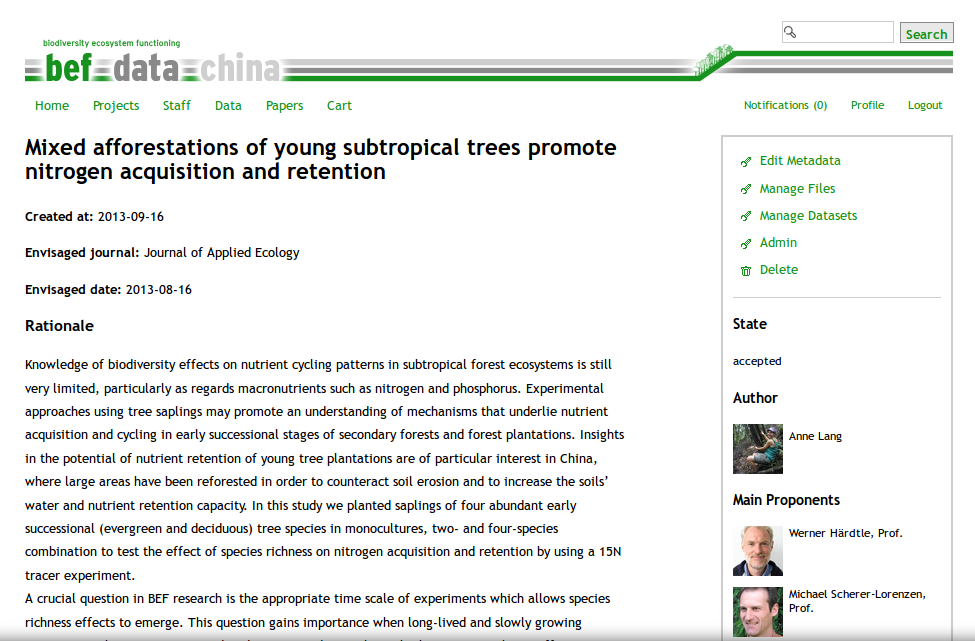
\includegraphics{./figure/static/showcase_proposal.png}
\caption{showcase\_proposal}
\end{figure}

\subsubsection{rbefdata}

The \texttt{rbefdata} package started its development within the
BEF-Cina experiment. Meanwhile it is part of the rOpenSci package
porfolio (http://ropensci.org/), which is a community driven approach to
wrap all science APIs and to create solutions to pull data from
different repositories into R for analysis.

The package can be installed from the CRAN package repository
(https://github.com/befdata/befdata) and enables access to the data,
meta data structures of the platform and provides convenient methods to
pull single or multiple dataset into the R environment in one step for
analysis.

Additionally it offers functions that help to upload final results
datasets with the script attached that has been used to derive the
results from the original datasets which provides a valuable insight
into data provenance and also is a stepping stone for reproducible
research.

\subsection{Usecase (results)}

First steps after the paper proposal are to setup the rbefdata package
for work. This requires loading the package and to set the package
options that are required so it works properly. Having a look into the
options list reveals several fields that can be filled in like the URL
to the BEFdata server, user credentials and a download folder that is
used to store downloaded freeformat files. The tematres server related
URLs are already part of upcomming features and will be of no special
interest for the workflow we present. The most essential setting for the
workflow we show here is the user credentials. These are used to
authenticate the user against the portal to ensure the access to the
data has been granted and to log the data access so. Setting the URL is
not required in this case as it defaults to the BEF-China project
instance of the BEFdata portal. If one has set up an own instance of the
BEFdata portal, this URL needs to be changed so the package communicates
with the right server.

\begin{Shaded}
\begin{Highlighting}[]
\KeywordTok{require}\NormalTok{(rbefdata)}
\CommentTok{# options list}
\KeywordTok{bef.options}\NormalTok{()}
\end{Highlighting}
\end{Shaded}

\begin{verbatim}
## $url
## [1] "http://china.befdata.biow.uni-leipzig.de"
## 
## $tematres_url
## [1] "http://tematres.befdata.biow.uni-leipzig.de/vocab/index.php"
## 
## $tematres_service_url
## [1] "http://tematres.befdata.biow.uni-leipzig.de/vocab/services.php"
## 
## $download_dir
## [1] "downloads"
## 
## $user_credentials
## [1] ""
\end{verbatim}

\begin{Shaded}
\begin{Highlighting}[]

\CommentTok{# querry single options}
\KeywordTok{bef.options}\NormalTok{(}\StringTok{"url"}\NormalTok{)}
\end{Highlighting}
\end{Shaded}

\begin{verbatim}
## [1] "http://china.befdata.biow.uni-leipzig.de"
\end{verbatim}

\begin{Shaded}
\begin{Highlighting}[]
\CommentTok{# set credentials example}
\KeywordTok{bef.options}\NormalTok{(}\DataTypeTok{user_credentials =} \StringTok{"aölkjspoiul12"}\NormalTok{)}
\end{Highlighting}
\end{Shaded}

\begin{Shaded}
\begin{Highlighting}[]
\CommentTok{# set URL example}
\KeywordTok{bef.options}\NormalTok{(}\DataTypeTok{url =} \StringTok{"http://my.own.befdata.instance.com"}\NormalTok{)}
\end{Highlighting}
\end{Shaded}

After setting up the \texttt{rbefdata} package we can start right away
using the data from the proposal. The proposal download method is used
for that which we need to provide with ID of the proposal. It draws all
associated datasets in one step into the R environment so we can work
with it. The ID of the proposal can be found in its URL.

\begin{verbatim}
# the id is 90
http://befdataproduction.biow.uni-leipzig.de/paperproposals/90
\end{verbatim}

\begin{Shaded}
\begin{Highlighting}[]
\CommentTok{# proposal id is}
\NormalTok{dataset_list = }\KeywordTok{bef.get.datasets_for_proposal}\NormalTok{(}\DataTypeTok{id =} \DecValTok{90}\NormalTok{)}
\NormalTok{extract_one_dataset = dataset_list[[}\DecValTok{1}\NormalTok{]]}
\end{Highlighting}
\end{Shaded}

\begin{itemize}
\itemsep1pt\parskip0pt\parsep0pt
\item
  Inspect datasets
\item
  after download (attributes())
\item
  in general bef.get.metadata\_for(dataset = id)
\end{itemize}

As the BEFdata portal provides metadata via EML we also make use of it
within the rbefdata package. Each dataset is associated with its
metadata available on the portal on download. It can be extracted using
the built-in R function \texttt{attributes()} like shown in code box
xxx. As this requires access to the dataset, there is also a function
especially to only draw metadata with is always free for download.

\begin{Shaded}
\begin{Highlighting}[]
\KeywordTok{attributes}\NormalTok{(dataset_list[[}\DecValTok{1}\NormalTok{]])$title}
\end{Highlighting}
\end{Shaded}

\begin{verbatim}
## [1] "Competition of saplings for N -Pilot- 15N recovery in leaves and fine roots "
\end{verbatim}

\subsection{Discussion}

\begin{itemize}
\item
  General discussion
\item
  high need to effective use/reuse data
\item
  relevant data needs to be simply detectable
\item
  BEFdata and rbefdata
\item
  in combination provide a solution to

  \begin{itemize}
  \itemsep1pt\parskip0pt\parsep0pt
  \item
    data storage
  \item
    describing data with metadata
  \item
    collaboration and data sharing
  \item
    simply pull data into analysis software and push data back
  \item
    data provenance by attaching R scripts to uploads
  \end{itemize}
\item
  will provide solution with next versions

  \begin{itemize}
  \itemsep1pt\parskip0pt\parsep0pt
  \item
    easier finding relevant data
  \item
    smart merges (including unit conversions)
  \end{itemize}
\end{itemize}

As there is a growing demand to effectively reuse available data this
puts much pressure on the development of solutions that help researchers
not only to find but also to integrate heterogeneous small data into a
wider context of in different analyses (cite xxx, data intensive
science, long tail). The combination of BEFdata and the rbefdata package
provides a solutions to a one part of the data life cycle and especially
introduces a solution to deal with high heterogeneous data.

We recently stared to develop an ontology using a tematres server
containing knowledge extracted from portals that deal with data
management for ecological research. The tematres server offers an API so
all the contained terms can be accessed by the upcoming version of
rbefdata

The formalization developed is and will be based on the knowledge used
in biodiversity research. Thus we will here discuss the software
combination BEFdata and rbefdata in the light of the upcoming features
and in general context state of the art data management today. In one of
the next versions to be rolled out the BEFdata portal will get a
semantical annotation feature. This will give admins and data admins the
ability to tag each column of datasets with a general term that best
describes the content. So the field will contain top terms of the
ontology. The tagging will be reflected in the API and can thus be
simply queried to use the information within the R package. Using the
knowledge about the content of a column in the R package will enable us
to do support smart merges that work

\texttt{tematres}
(\href{http://www.vocabularyserver.com/}{homepage})into BEFdata and the
rbefdata package so they play well together semantically.

\subsection{Acknowledgements}

Thanks to all the data owners of the proposal for providing access to
the datasets. \ldots{}

\subsection{Literature}

This will be done externally as markdown has no good way to deal with
references and stuff. We can collect here a list of links to references.
I will then collect them with e.g zotero to export a format we can hand
them in for publication.

\subsection{Appendix}

\begin{itemize}
\itemsep1pt\parskip0pt\parsep0pt
\item
  maybe will not be used extensively but we will see
\end{itemize}

\subsubsection{Figures}

\begin{itemize}
\itemsep1pt\parskip0pt\parsep0pt
\item
  vizualization plugin (keywords)
\end{itemize}

One can visualize the keywords associated with the dataset of a BEFdata
portal using the vitalization functionality. This gives a short overview
about the contents the portal data is dealing with.

\begin{Shaded}
\begin{Highlighting}[]
\KeywordTok{bef.portal.vizualize.keywords}\NormalTok{()}
\end{Highlighting}
\end{Shaded}

\begin{figure}[htbp]
\centering
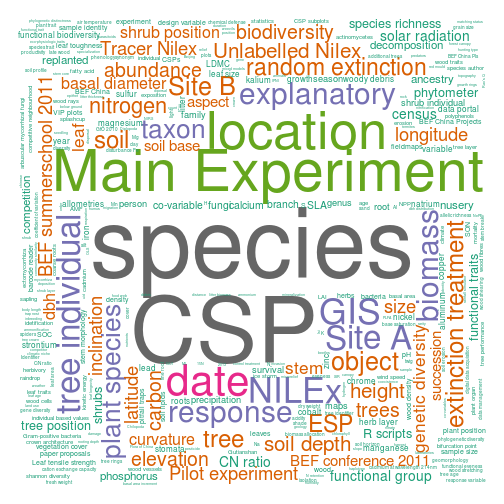
\includegraphics{figure/vizalize_keywords.png}
\caption{plot of chunk vizalize\_keywords}
\end{figure}

\subsubsection{Tables}

\end{document}
